\chapter{NoSQL}
\begin{nota}
      In quest capitolo non si vuole sostenere che i database NoSQL siano
      migliori di quelli relazionali. I database NoSQL sono un'alternativa
      ai database relazionali e non sempre sono la scelta migliore. Per ogni
      applicazione è necessario valutare quale sia la scelta migliore.
\end{nota}
Fino a questo momento abbiamo utilizzato database relazionali per gestire le
nostre applicazioni. Tuttavia, i database relazionali non sono l'unica
opzione disponibile. In questo capitolo, esploreremo un'alternativa ai
database relazionali: i database NoSQL.
\section*{Use Cases}
\subsection*{Crypto}
Iniziamo analizzando il seguente Use Case: un cliente vuole salvare dati legati
alle crypto che vengono forniti da un API. Con le conoscenze conseguite fino a
questo momento, salveremo tutto su una tabella di un DBMS relazionale dove si
hanno 5 colonne:
\begin{itemize}
      \item id
      \item Simbolo
      \item Prezzo\_USD
      \item Prezzo\_EUR
      \item Data
\end{itemize}
Questa soluzione presenta dei problemi, ad esempio, se si volesse salvare
informazioni aggiuntive o se la risposta dell'API si dovesse modificare, si
dovrebbe modificare la tabella. Un altro problema sorge quando nella risposta
sono contenuti elementi complessi, come ad esempio un array di oggetti. In questa
situazione, usando un database relazionale, si dovrebbero creare tabelle diverse
e ogni volta che si vuole fare una nuova interrogazione è necessario fare delle
join tra le tabelle. Questo comporta un rallentamento delle prestazioni.

Una soluzione per ridurre il numero di join è quello di duplicare i dati, il
problema in questo caso non è più legato alla velocità delle interrogazioni, ma
al mantenere la consistenza dei dati.

In aggiunta posso ridurre le tabelle unendole creando una grande tabella che può
essere frammentata a livello fisico, il problema di questa soluzione è che si
vanno a inserire un elevato numero di valori \texttt{null}.
\subsection*{Social network}
Un altro caso d'uso è il social network in cui si vuole salvare la relazione di
amicizia tra profili, il problema è che se si avessero 1M di utenti, ciascuno con
100 amici, allora la tabella amicizia diventa 100M di record. Troppa complessità
soprattutto per una tabella che verrà usata spesso con delle join.

Il DB relazionali non sono in grado di modellare efficientemente i contesti applicativi
con volumi molto significativi di dati.
\section{Introduzione}
Da questo use case possiamo osservare che il modello relazionale presenta dei
limiti nella gestione dei dati:
\begin{itemize}
      \item Si ha uno svantaggio nel salvare di dati poco omogenei, questo è dovuto
            principalmente alla rigidità dello schema dei modelli relazionali, in
            quanto prima di poter inserire i dati, è necessario definire la loro
            struttura.
      \item Si ha uno svantaggio in relazione al paradigma di programmazione che
            viene usato (Programmazione a oggetti). Questo obbliga a utilizzare
            un ORM per mappare i dati del database relazionale con gli oggetti
            del linguaggio di programmazione.
\end{itemize}
Inoltre, essendo le risposte delle API solitamente in formato JSON, si ha un
ulteriore svantaggio in quanto si deve fare un parsing della risposta per
poterla salvare nel database relazionale.

I database NoSQL sono nati con lo scopo di risolvere alcuni problemi di quelli
relazionali come la scalabilità e la flessibilità. Inoltre, le assunzioni che
si trovano dietro i database relazionali non sono sempre adatte per tutti i
casi d'uso.

Con questo non vogliamo dire che i database NoSQL siano migliori di quelli
relazionali, ma che sono un'alternativa ai database relazionali. Per ogni
applicazione è necessario valutare quale sia la scelta migliore. Di seguito
elenchiamo alcuni motivi per cui utilizzare i database relazionali:
\begin{itemize}
      \item SQL è semplice.
      \item Molto rigido
      \item Vincoli nel database allora le app possono non fare i controlli
      \item ipotesi di mondo chiuso: tutto quello che serve è nel database, se non
            lo so devo inserire il valore \texttt{null}.
      \item Tecnologia stabile e funzionante che alle spalle anni di ricerca e
            sviluppo.
      \item Sono valide le proprietà ACID, molto utili in contesti in cui si
            hanno transazioni.
\end{itemize}
È corretto presentare anche gli svantaggi dei database relazionali:
\begin{itemize}
      \item Modificare una tabella nella quale sono già presenti dei valori è molto
            complicato.
      \item Assunzione mondo chiuso: può risultare troppo pesante in determinate
            situazioni.
      \item Il concetto di minimizzare le ripetizioni dei valori implica la necessità
            di effettuare molte join per ottenere l'informazione desiderata.
      \item Si ha un mapping un attributo ha un valore.
      \item Non è compatibile con i linguaggi di programmazione ad oggetti.
      \item Presenta delle difficoltà nella gestione dei self-join.
      \item È difficilmente scalabile.
\end{itemize}
\begin{nota}
      Il termine NoSQL significa \textit{Not Only SQL}.
\end{nota}
Una caratteristica comune dei database NoSQL è che sono \textbf{schema-free} o
\textbf{schema-less}. Questo significa che non è necessario definire uno schema
prima di poter inserire i dati. L'inserimento dei dati implica per quel dato lo
schema associato, il successivo inserimento di un dato può avere uno schema diverso.

% Presa da internet la definizione
Oltre a ciò, per questi database vale il \textbf{teorema CAP}, il quale afferma
che è impossibile per un sistema distribuito garantire contemporaneamente le
seguenti tre proprietà:
\begin{itemize}
      \item \textbf{Consistency}: tutti i nodi vedono gli stessi dati allo stesso
            tempo.
      \item \textbf{Availability}: ogni richiesta riceve una risposta, anche in
            presenza di guasti.
      \item \textbf{Partition tolerance}: il sistema continua a funzionare anche
            se alcune parti del sistema non sono disponibili.
\end{itemize}
Mentre nei database relazionali avevamo le transazioni \textbf{ACID}, nei database
NoSQL abbiamo le transazioni \textbf{BASE}, che stanno per:
\begin{itemize}
      \item \textbf{Basically Available}: il sistema è sempre disponibile.
      \item \textbf{Soft state}: lo stato del sistema può cambiare anche senza
            input.
      \item \textbf{Eventual consistency}: il sistema diventerà consistente in un
            certo momento.
\end{itemize}

Inoltre, a differenza dei database relazionali, i database NoSQL si basano su
un'assunzione di mondo aperto, ovvero viene inserito solo quello che conosco se
mi mancano delle informazioni non le metto.

Si è passati dal progettare le architetture in modo da essere più specifiche
per l'applicazione, il contrario di come si faceva una volta: progettazione generalista.
\section{Tipi di database NoSQL}
Esistono diverse tipologie di database NoSQL, ognuna con le proprie caratteristiche
e i propri casi d'uso. Possiamo dire che più è semplice il modello, più è facile
scalarlo. Nella figura \ref{fig:tipi_nosql} possiamo osservare come si posizionano i
database NoSQL rispetto alla dimensione e complessità del modello.
\begin{figure}[!ht]
      \centering
      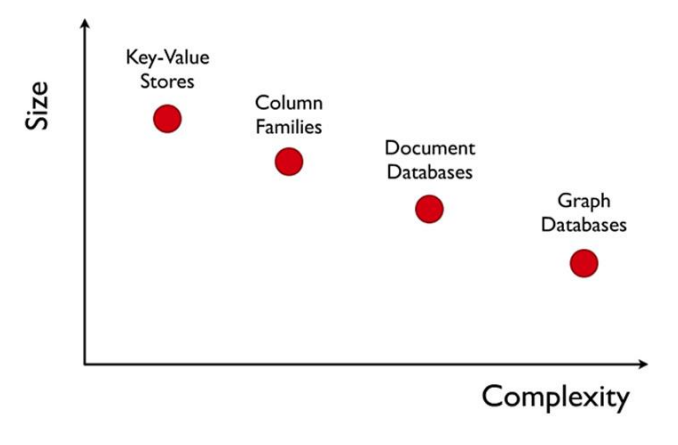
\includegraphics[scale=0.5]{./img/nosql/tipi_nosql.png}
      \caption{Tipi di database NoSQL}
      \label{fig:tipi_nosql}
\end{figure}

Rispetto questa rappresentazione possiamo posizionare il modello relazionale tra
il modello column-based e il modello document-based.

In questo corso vedremo i seguenti tipi di database NoSQL:
\begin{itemize}
      \item \textbf{Document-based}: i dati sono memorizzati in documenti, che
            possono essere in formato JSON, XML, BSON, YAML, etc.
      \item \textbf{Key-value}: i dati sono memorizzati in coppie chiave-valore.
      \item \textbf{Wide-column}: i dati sono memorizzati in colonne, simile ai
            database relazionali.
      \item \textbf{Graph-based}: i dati sono memorizzati in nodi e archi.
\end{itemize}
Una caratteristica che accomuna queste tipologie di database è legata al problema
di mettere insieme i dati. Ad esempio, i database relazionali usano le operazioni
di join, mentre i database document-based usano un unico documento.
\subsection{Key value}
I database \textbf{key-value} sono i più semplici tra i database NoSQL. In questi
database, i dati sono memorizzati come tabelle di hash dove la chiave punta a un
particolare valore. Si utilizzano le tabelle di hash per massimizzare le prestazioni
di lettura e scrittura.
\subsection{Wide column}
I database \textbf{wide-column} sono simili ai database relazionali, ma invece di
memorizzare i dati in righe, i dati sono memorizzati in colonne. Questo permette
di avere una maggiore flessibilità rispetto ai database relazionali. La chiave
punta a un insieme di colonne che può essere diverso per ogni riga.

\paragraph{HBASE}
HBase è un database wide-column che è stato ispirato da Google BigTable. In HBase
si ha una chiave che punta ad un insieme di valori che possono avere tipi differenti.

In questa struttura, possiamo definire delle \textbf{column family}, le quali
contengono più attributi che condividono delle informazioni. Il \textbf{qualifier} è
il nome dell'attributo all'interno di una column family. Ogni riga ha anche
un campo relativo al timestamp in cui è stata modificata.

L'utilizzo di timestamp fornisce un modo diverso per gestire le transazioni,
anche quelle distribuite, senza l'uso di lock. Questo metodo associa a ogni
transazione un timestamp, in modo che se due transazioni si sovrappongono,
possono essere risolte in base a tale valore.

In questa implementazione è possibile realizzare facilmente relazioni di tipo 1-n
nella stessa riga.
\paragraph{Cassandra}
Cassandra è un database wide-column che è stato realizzato da Facebook per gestire
la comunicazione con le mail.

Questo database si differenzia da HBase per il fatto si ha uno spazio delle chiavi,
il quale può essere visto come una tabella nel modello relazionale. Questo spazio
è suddiviso in column family, le quali sono differenti da quelle di HBase in quanto
la stessa chiave primaria può essere usata in più column family.

I valori che si trovano all'interno di una column family possono essere di tipo
diverso, inoltre, ogni riga ha un timestamp associato.

Quindi una column family equivale ad una \textit{tabella}, e si utilizza la chiave
primaria della riga per accedere ad un particolare dato di essa.

L'accesso viene effettuato specificando i seguenti campi:
\begin{itemize}
      \item \texttt{column family}
      \item \texttt{row key}
      \item \texttt{column name}
\end{itemize}
Per semplificare il passaggio da database relazionali a Cassandra, il query
language di Cassandra (CQL) è molto simile a SQL. Attraverso questo meccanismo
è possibile sviluppare un applicazione che è in grado di utilizzare sia database
relazionali che Cassandra senza apportare molte modifiche.

Un vantaggio dell'utilizzo di questo database è legato al fatto che ogni riga è
indipendente dalle altre. Quindi, in un contesto distribuito, è possibile frammentare
come si vuole il database senza dover fare join.
\subsection{Document based}
I database \textbf{document-based} permettono di memorizzare delle informazioni sotto
forma di documenti. Ognuno dei quali è identificato attraverso una chiave unica.
Tutte le operazioni di lettura e manipolazione dei dati avvengono all'interno
dei documenti stessi.
\paragraph{MongoDB}
MongoDB è un database document-based che memorizza i dati in documenti JSON, più
precisamente, utilizza un formato binario di JSON chiamato BSON. Ogni documento
è identificato da una chiave unica, chiamata \texttt{\_id}.

Possiamo immaginare la struttura di un file JSON come un albero, dove la radice
è la chiave \texttt{\_id} e i figli sono i campi del documento.

Questa tipologia permette di salvare i dati come si faceva negli schemi relazionali,
ovvero suddividendo le informazioni in diverse \textbf{collezioni}. Per fare ciò,
si utilizzano i \textbf{riferimenti} tra i documenti. Lo svantaggio di questa
soluzione è che si devono fare molte join per ottenere l'informazione desiderata.

Un'altra soluzione è quella di salvare i dati in un unico documento, sfruttando
l'embedding, in modo da evitare le join. Questo metodo è molto efficiente quando
si devono accedere alle informazioni più vicine alla radice, ma meno efficiente
quando si devono accedere alle foglie, si ha comunque un tempo di accesso minore
rispetto alle join.

Nei database document-based lo schema non è vincolante, in particolare, corrisponde
all'unione di tutti gli attributi e sotto-attributi del documento.

Vediamo ora un parallelismo tra i database relazionali e MongoDB:
\begin{itemize}
      \item \textbf{Database} $\rightarrow$ \textbf{Database}
      \item \textbf{Tabella} $\rightarrow$ \textbf{Collection}
      \item \textbf{Row} $\rightarrow$ \textbf{Document}
      \item \textbf{Column} $\rightarrow$ \textbf{Field}
      \item \textbf{Index} $\rightarrow$ \textbf{Index}
      \item \textbf{Join} $\rightarrow$ \textbf{Embedded document}
      \item \textbf{Foreign key} $\rightarrow$ \textbf{Reference}
      \item \textbf{Partition} $\rightarrow$ \textbf{Shard}
\end{itemize}
Le operazioni che si vogliono svolgere sulla base di dati vengono espresse
attraverso una notazione che ricorda quella della programmazione a oggetti, ovvero
attraverso la \textit{dot notation}. Inoltre, nelle operazioni tutti gli
operatori devono essere espressi in JSON. Questo permette di eliminare l'utilizzo
di framework come Hibernate per mappare gli oggetti sul database.
\begin{nota}
      Quando si devono caricare grandi quantità di dati è utile disabilitare
      l'ack che viene mandato per ogni operazione.
\end{nota}
Le query di modifica di un documento presentano degli oggetti JSON come
clausole, simile alla clausola \texttt{WHERE} delle query SQL. Oltre a questo
è possibile specificare di creare un documento nuovo nel caso non sia presente
quello che si vuole modificare.

Mongo permette di creare degli indici per velocizzare le operazioni.
\begin{esempio}
      Vediamo ora un esempio di parallelismo tra una query SQL e una per
      MongoDB:
      \begin{center}
            db.\textcolor{red}{users}.find(\textcolor{green}{\{age: \{ \$gt: 18 \}\}},
            \textcolor{cyan}{\{name: 1, age: 1\}}).\textcolor{magenta}{limits(10)}
      \end{center}
      \begin{center}
            \textcolor{cyan}{SELECT name, age} \textcolor{red}{FROM users}
            \textcolor{green}{WHERE age $>$ 18} \textcolor{magenta}{LIMIT 10}
      \end{center}
\end{esempio}
Nelle interrogazioni, tutte le clausole sono specificate in \texttt{AND}, se si
vuole specificare in \texttt{OR} è necessario utilizzare il comando \$$or$ seguito
      da una lista di oggetti JSON.

      Nelle versioni successive è stato definito il concetto di \textbf{aggregation} e
      di \textbf{pipeline}. Una pipeline è un comando che rappresenta una sequenza di
      operazioni che vengono eseguite in serie e possono essere usate per operazioni
      di analytics.

      \begin{nota}
            Dato un problema non sempre per avere efficienza dobbiamo scegliere la
            soluzione banale, spesso dobbiamo prendere soluzioni controintuitive. Ex:
            salvare i dati non in modo efficiente e sfruttare la potenza di esecuzione
            delle query dei DBMS.
      \end{nota}
      \begin{nota}
            Un documento è un albero.
      \end{nota}
      \subsection{Graph based}
      I database graph-based memorizzano i dati salvando le informazioni nei nodi e
      utilizzando gli archi per definire delle relazioni tra esse. Questi database sono
      utili per memorizzare dati che hanno relazioni complesse, come ad esempio le
      relazioni dei social network.

      Spesso si usano per reti sociali, recommendations systems, logistica, financial
      transaction, bioinformatica, autorizzation and access control.

      I database basati sui grafi godono delle seguenti proprietà:
      \begin{itemize}
            \item \textbf{Storage}:
                  \begin{itemize}
                        \item \textbf{Nativo}: i dati vengono salvati sotto forma di
                              grafo, si ha la problematica legata alla scalabilità
                              della soluzione.
                        \item \textbf{Non nativo}: i dati vengono salvati in una struttura
                              differente da un grafo, ma che logicamente permette di essere
                              visto come un grafo.
                  \end{itemize}
            \item \textbf{Processing engine}:
                  \begin{itemize}
                        \item \textbf{Nativo}: permette di effettuare direttamente query
                              nel linguaggio dei grafi, sfruttando le proprietà dei
                              grafi. Il problema di questa soluzione è dovuto al fatto
                              che bisogna mappare le query reali utilizzando le proprietà
                              del grafo.
                        \item \textbf{Non nativo}: permette di utilizzare un altro
                              linguaggio (es. SQL) per effettuare query che non devono
                              per forza essere proprietà del grafo.
                  \end{itemize}
      \end{itemize}
      Lo storage nativo, spesso si basa sull'\textbf{index friend adjacency}, ovvero
      i nodi che sono vicini sono fisicamente salvati insieme. Questo permette di
      effettuare query molto velocemente, ma la costruzione del grafo è molto lenta.

      Il collegamento tra concetti si effettua attraverso un cammino tra nodi, mentre
      nel relazionale si effettua tramite valori, invece nel documentale si usa l'embedding.

      La struttura a grafo dei dati permette di rappresentare le informazioni
      attraverso un database documentale, ma essendo la base di tale modello una
      struttura ad albero risulta più complesso mappare le relazioni tra i dati.
      Per risolvere questo problema si utilizzando i riferimenti tra vari documenti.

      Un modo efficiente per modellare un grafo in modo non nativo è quello di sfruttare
      i vicini. Ad esempio, in un modello documentale possiamo utilizzare l'embedding
      per memorizzare i nodi vicini, mentre per i nodi lontani possiamo utilizzare i
      riferimenti.

      Una seconda soluzione è quella di usare relazioni differenti nel grafo per aumentare
      l'espressività del grafo e semplifica i collegamenti. Questo può essere implementato
      facilmente.

      \begin{esempio}
            Metti l'esempio del confronto delle interrogazioni tra modelli.
      \end{esempio}

      Nel modello a grafo, ogni nodo rappresenta le informazioni al suo interno con
      delle proprietà, ovvero coppie chiave-valore dove la chiave è rappresentata
      dall'etichetta e il valore rappresenta l'informazione. Anche le relazioni possono
      avere un etichetta a cui è associata una proprietà.

      Una stessa informazione può essere modellata in modi diversi, la scelta dipende
      dalle query che si vogliono effettuare. Le due soluzioni sono:
      \begin{itemize}
            \item \textbf{Stessa etichetta}: si ha una sola etichetta per accedere
                  a tutte le informazioni, mentre all'interno della relazione si specifica
                  il tipo di informazione.
            \item \textbf{Etichette multiple}: si ha una relazione per ogni tipo di
                  informazione.
      \end{itemize}
      Ad esempio, per modellare una situazione in cui a una persona sono associati più
      indirizzi, si possono utilizzare le due soluzioni, la scelta dipende dalle
      tipologie di query che si vogliono effettuare. Se si vogliono trovare tutti
      gli indirizzi di una persona, allora è meglio utilizzare una soluzione in cui
      si ha una stessa etichetta per accedere a tutti gli indirizzi e poi all'interno
      della relazione si specifica il tipo di indirizzo. Mentre, se si vogliono
      effettuare query per sapere uno specifico tipo di indirizzo è più conveniente
      utilizzare una relazione per ogni tipo di indirizzo.
      \paragraph{Query language}
      La modellazione tramite grafo risulta semplice a livello semantico da costruire,
      il problema è che non si ha uno standard per il Query language, eccone alcuni:
      \begin{itemize}
            \item \textbf{Cypher}: linguaggio dichiarativo basato sul \textbf{
                        pattern-matching query language} (come SQL), infatti
                  cerca tutti i sottografi che metchano con il grafo di query.
                  Permette di effettuare aggregation, ordering e limit.

                  Il risultato di una query grafo può essere una tabella o un
                  sottografo. La notazione di Cypher è la seguente:
                  \begin{center}
                        \texttt{(nodo)-[:etichetta]->(nodo2)}
                  \end{center}
                  Mettendo più condizioni separate dalla virgola equivale a
                  considerarle in and. Vediamo ora un esempio di query in Cypher:
                  \begin{lstlisting}[language=SQL]
                        MATCH (n:Person)-[r:KNOWS]->(m:Person)
                        WHERE n.name = 'Alice'
                        RETURN m.name
                  \end{lstlisting}
            \item \textbf{Gremlin} (graph traversal language): la query consiste
                  nel specificare un percorso. Il percorso viene inizializzato in
                  tutti i nodi. Nella query è possibile specificare dei constrain
                  su archi e nodi per selezionare quali percorsi considerare.

                  Questo linguaggio è pensato per essere eseguito ad agenti,
                  quindi è parallelizzabile ed eseguibile in ambienti distribuiti.

                  Vediamo un esempio di query in Gremlin:
                  \begin{lstlisting}[language=SQL]
                        g.V().has('name', 'Marko').out('KNOWS').values('name')
                  \end{lstlisting}
      \end{itemize}

      \section{Modelli poliglotti}
      Esistono delle soluzioni che integrano più modelli di database in un unico
      sistema, queste soluzioni sono chiamate modelli poliglotti.

      Un esempio di modello poliglotta è \textbf{ArangoDB}, un DBMS che supporta i
      seguenti modelli:
      \begin{itemize}
            \item \textbf{keyvalue}
            \item \textbf{graph}
            \item \textbf{document}
            \item \textbf{ricerca full text}
      \end{itemize}
      Tutti i modelli sono gestiti come documenti JSON, più precisamente si hanno due
      documenti principali:
      \begin{itemize}
            \item \textbf{databases} (schemas): contengono lo schema generico delle collections
            \item \textbf{collections} (tables): contengono documenti JSON di tipi simili
      \end{itemize}
      In questo modo si possono facilmente gestire i modelli key-value. Per quanto riguarda
      il graph model, in questo caso ArangoDB utilizza una collection per specificare
      i nodi, ciascun nodo viene descritto da un documento JSON. Successivamente si
      rappresentano i collegamenti utilizzando una nuova collection che contiene un documento
      JSON per ogni arco. Il documento contiene gli indici dei due nodi e quindi si effettua
      il referencing tra documenti. In fase di query si effettuerà la Join per collegare
      i nodi agli archi.
      \section{Distribuited NoSQL}
      I sistemi RDBMS sono facilmente scalabili verticalmente (\textbf{Scale up}),
      ovvero si potenzia la singola macchina, ma non sono facilmente scalabili
      orizzontalmente (\textbf{scale out}), il che consiste nell'aggiungere nodi
      all'infinito al cluster.

      Questo vincolo è dovuto alle proprietà ACID che devono essere rispettate per
      definizione. Questo non è un problema per i database NoSQL, in quanto sono
      progettati per essere scalati orizzontalmente. Infatti, per questi database vale
      il CAP theorem, il quale afferma che:
      \begin{teorema}[\textbf{CAP theorem}]
            In un sistema distribuito non è possibile garantire contemporaneamente
            le tre proprietà seguenti:
            \begin{itemize}
                  \item \textbf{Consistency}: tutti i nodi vedono gli stessi dati
                  \item \textbf{Availability}: ogni richiesta riceve una risposta
                  \item \textbf{Partition tolerance}: il sistema continua a funzionare
                        anche in presenza di partizioni di rete
            \end{itemize}
            al massimo due di queste proprietà possono essere garantite contemporaneamente.
      \end{teorema}
      Con la nuova scoperta si ogni DBMS si è incentrato su solo 2 proprietà di quelle
      descritte. Generalmente i RDBMS rispettano CA, mentre per i NoSQL, per via delle
      proprietà BASE, non si limitano alla combinazione di solo CA. Con queste considerazioni
      i sistemi NoSQL sono più facili da scalare (vedi figura \ref{fig:cap}).
      \begin{figure} [!ht]
            \centering
            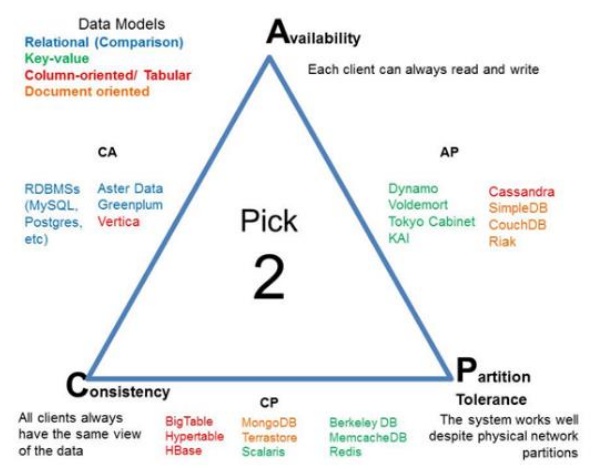
\includegraphics[width=0.5\textwidth]{img/nosql/CAP.png}
            \caption{DBMS con le proprietà che assicurano di rispettare}
            \label{fig:cap}
      \end{figure}
      Oltre a questo teorema, i modelli NoSQL si basano sul principio \textbf{BASE},
      ovvero:
      \begin{itemize}
            \item \textbf{Basically Available}: il sistema garantisce una disponibilità
                  di servizio anche in presenza di fallimenti
            \item \textbf{Soft state}: lo stato del sistema può cambiare anche in assenza
                  di input
            \item \textbf{Eventually consistent}: il sistema raggiunge uno stato consistente
                  in un certo momento, anche se non è garantito che lo sia in ogni momento
      \end{itemize}
      \subsection{Keyvalue model: Redis}
      Redis essengo un keyvalue non effettua frammentazione, permette di creare dei
      cluster con più nodi e permette di implementare meccanismi automatici e trasparenti
      di replica per avere alta Availability.

      La replica può essere implementata a livello di cluster, si utilizza un cluster
      "Master" di nodi su cui si effettuano le letture e le scritture, successivamente
      si utilizzano dei cluster "Slave" di nodi su cui si effettua la replica dei cluster
      "Master", questi vengono usati principalmente in lettura. Un'altra implementazione
      è tramite la definizione delle repliche sugli stessi nodi del cluster, questo
      comporta che non abbiamo meccanismi Master-slave a livello di cluster, bensì a
      livello di nodi. Quindi per ogni cluster possiamo sia leggere sia scrivere
      (vedi \ref{fig:dist_redis}).
      \begin{figure} [!ht]
            \centering
            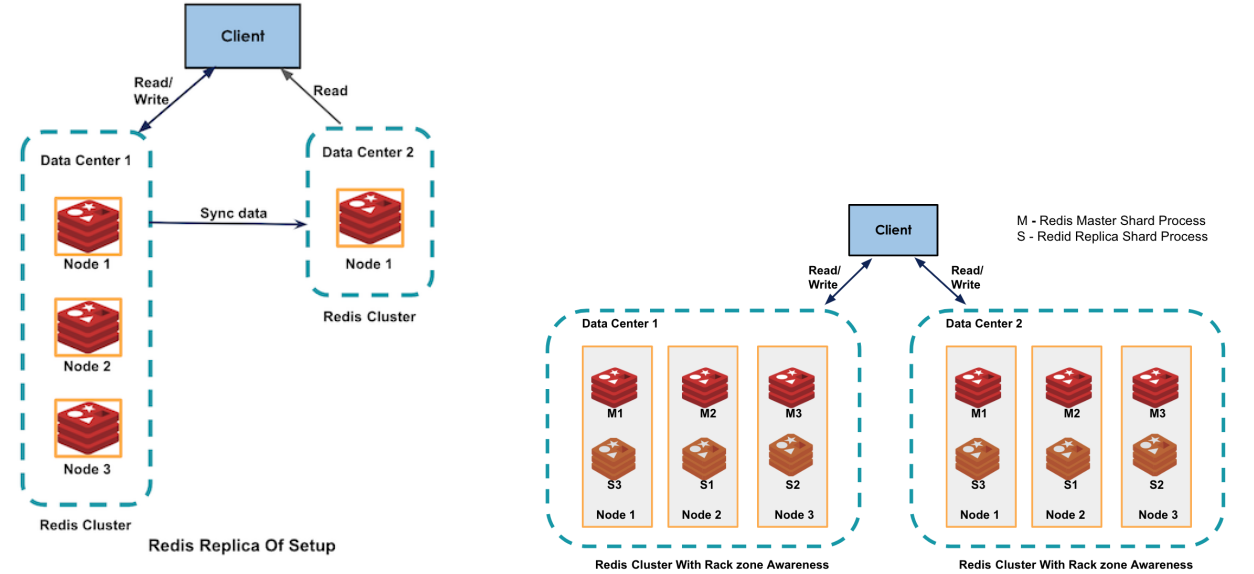
\includegraphics[width=0.5\textwidth]{img/nosql/redis_distribuited.png}
            \caption{Due metodologie per replicare con Redis}
            \label{fig:dist_redis}
      \end{figure}

      Le shard create possono essere:
      \begin{itemize}
            \item \textbf{Dense}: se un nodo ha abbastanza memoria allocata per il
                  database, allora le shard possono essere posizionate sullo stesso nodo
                  e solamente dopo che è pieno si passa a un nuovo nodo.
            \item \textbf{Sparse}: viene utilizzato il massimo numero di nodi per
                  distribuire le shard.
      \end{itemize}
      \subsection{Column Family model: HBASE}
      La distribuzione con HBase si basa sul meccanismo Master-slave e sulla frammentazione
      orizzontale, ciascun frammento si chiama \textbf{Region}.

      La distribuzione si basa su 2 componenti:
      \begin{itemize}
            \item \textbf{HBase master}: è un'istanza di HBase che si occupa di
                  coordinare gli slave, assegna i region agli slave e riconosce i
                  fallimenti. Permette inoltre di effettuare operazioni di admin.
            \item \textbf{Region server}: sono le singole istanze slaves del cluster,
                  si occumano di salvare effettivamente i region assegnati dal master
                  e si occupa di gestirli, fornisce le funzioni di lettura e scrittura
                  dei suoi region tramite i log. Su ogni Region server si possono
                  implementare meccanismi di replica.
            \item \textbf{Hbase Client}: è il client che dialoga con il master per fare le
                  richieste.
      \end{itemize}
      Il cluster sarà formato da un nodo HBase master e tanti Region Server, quest'ultimi
      possono avere diversi nodi per la replica. Nel cluster si avrà poi un'orchestratore
      (\textbf{ZooKeeper}) che permette il coordinamento tra Client, Master e Slaves
      in modo da risolvere eventuali problemi di fallimento (vedi \ref{fig:dist_hbase})
      \begin{figure} [!ht]
            \centering
            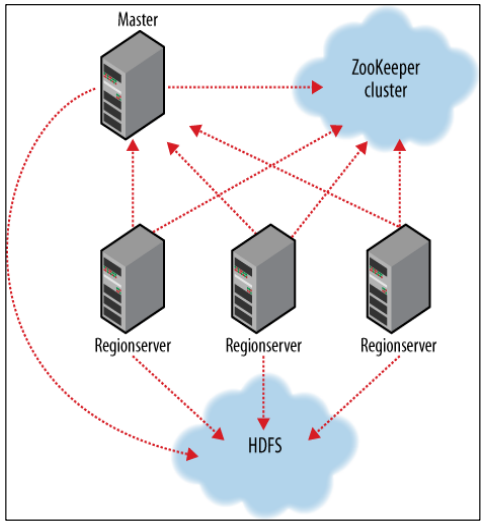
\includegraphics[width=0.4\textwidth]{img/nosql/hbase_distribuited.png}
            \caption{Architettura distribuita HBase}
            \label{fig:dist_hbase}
      \end{figure}
      \subsection{Column Family model: CASSANDRA}
      Cassandra distribuito ha un'architettura a cluster, ciascuno viene gestito in peer
      to peer con una rete ad anello. I dati vengono partizionati tra in nodi della rete e
      per risolvere i fallimenti si usa la replicaizone. Si scrive e legge su qualsiasi
      nodo, il numero di nodi del cluster può essere aggiornato a runtime.

      Le performance dipendono linearmente rispetto al numero di nodi.

      Essendo un'architettura peer-to-peer allora non ha single point of failure
      fornendo massima Availability. In aggiunta si può partizionare il database
      su più cluster differenti e separati geograficamente.

      Cassandra implementa anche la replicazione dei dati di un cluster in due modi:
      \begin{itemize}
            \item \textbf{Replicazione su un nodo}: si replicano i dati sullo
                  stesso nodo
            \item \textbf{Replicazione su un nodo diverso}: si replicano i dati su un
                  altro nodo dello stesso cluster. Questo permette di salvarsi dalla
                  perdita di dati se un nodo si guasta perché ci sarà una replica in
                  un altro nodo.
      \end{itemize}
      Si utilizzerà zookeeper per gestire le repliche, nota che le repliche devono essere
      almento $3$.

      Ogni cluster gestisce una partizione del database. Ognuna di queste presenta
      un ulteriore partizionamento dei dati, il quale viene gestito dai nodi interni.

      Il partizionamento avviene sfruttando funzioni di hashing. I nodi sono divisi in
      modo logico in una forma ad anello, detta ring topology. Si usano quindi i valori
      hash delle chiavi, associate alle partizioni dati, per assegnare l'informazione
      a uno dei nodi.

      Ciascun nodo viene posizionato nell'anello e gli viene associato un particolare
      valore, in questo modo ciascun nodo si occupa dei dati le cui funzioni di hash
      mappano l'informazione nella porzione di anello che va dal nodo precedente al
      nodo stesso.

      Quando si aggiunge un nuovo nodo si divide lo spazio di indirizzamento in modo
      da avere una distribuzione uniforme e i dati vengono replicati in modo automatico.

      Dal momento che si ha un'architettura peer-to-peer, per comunicare lo stato
      dei nodi e la locazione dei dati nel cluster si usa il \textbf{gossip protocol}.
      Questo protocollo permette di comunicare in modo efficiente tra i nodi, sfruttando
      il seguente meccanismo: se i dati non sono sul nodo attuale, allora si chiede a
      quelli adiacienti, i quali a loro volta controllano se hanno le informazioni. In
      caso contrario chiedono a quelli adiacienti, fino a quando non sono stati visitati
      tutti i nodi.

      Utilizzando il \textbf{gossip protocol} si può facilemnte \textbf{identificare
            il fallimento}, infatti, ogni nodo tiene salvato la sua probabilità di
      fallimento e in fase di comunicazione, in base alla velocità delle risposte
      aggiorna la sua probabilità, in questo modo si aumenta quando le condizioni
      della rete peggiorano, come la latenza ecc\dots

      Si usa una soglia che specifica sopra quanto la probabilità deve essere per considerare
      il nodo dead. Non si usa una politica basata sui timeout in quanto la rete può
      essere riempita di messaggi di gossip e quindi si può avere un ritardo.

      Le operazioni di scrittura su ciascun nodo seguono questi passi:
      \begin{itemize}
            \item Scrivo l'operazione nel LOG
            \item Scrivo il dato in RAM
            \item Quando i dati in RAM sono abbastanza scrivo su disco
      \end{itemize}

      Dal momento che si hanno partizioni e repliche in un particolare cluster, diventa
      fondamentale gestire la consistenza, in fase di query si deve specificare
      la tipologia di consistenza e il replication\_factor e successivamente in base
      alle operazioni si hanno diversi livelli di consistenza:
      \begin{itemize}
            \item scrittura:
                  \begin{itemize}
                        \item consistency one: si ritorna la risposta al client dopo una scrittura
                              su disco solo su un nodo del cluster
                        \item consistency all: si ritorna la risposta al client dopo una scrittura
                              su disco solo su un numero di nodi del cluster pari al replication factor
                        \item consistency quorum: si ritorna la risposta al client dopo $replication\_factor/2+1$ nodi che
                              hanno scritto su disco
                  \end{itemize}
            \item lettura:
                  \begin{itemize}
                        \item consistency one: si ritorna la risposta al client dopo la lettura
                              su un nodo del cluster
                        \item consistency all: si ritorna la risposta al client dopo una lettura
                              solo su un numero di nodi del cluster pari al replication factor
                  \end{itemize}
      \end{itemize}

      Le query di cancellazione vengono implementate attraverso le marcature che
      comunicano che il record è cancellato ma lo cancellano effettivamente in un secondo
      momento, più precisamente attraverso \textbf{major compaction} o dopo un timer.

      In merito alle operazioni di delete si ha che esse semplicemente rendono il
      dato non disponibile, essendo più veloce cambiare un flag piuttosto che cancellare.
      A causa di ciò comunque si creano nelle tabelle fisiche dei problemi di
      spazio, quindi periodicamente si fanno dei merge, ovvero ogni singolo nodo
      procede alla “compattazione” dei propri dati, sovrascrivendo i valori non più
      disponibili.

      Per assicurare la sincronizzazione dei nodi e per evitare perdita di consistenza
      si utilizzano dei checksum per comparare i dati di un nodo con quelli dei
      successivi. Per effettuare questo controllo, nel dettaglio, vengono usati degli
      hash-tree detti \textbf{Merkle tree} nel seguente modo:
      \begin{itemize}
            \item Vengono mandati degli snapshot dei dati ai nodi successivi.
            \item Vengono creati e trasmessi ad ogni “compattazione” principale.
            \item Se due nodi prendono uno snapshot con un intervallo pari a
                  \texttt{TREE\_STORE\_TIMEOUT} allora i due snapshot sono comparati e in
                  caso di successo i dati vengono sincronizzati.
      \end{itemize}
      Cassandra rientra nella catergoria AP.
      \subsection{Document model: MongoDB}
      MongoDB ha un'architettura master (primary) e slave (secondary). Si effettuano le
      scritture sul primary che poi replica sui secondary usando il file di LOG del primary.

      In sostanza ciascun cluster di nodi è chiamato shard, in ogni shard si identifica
      un nodo primary e tutti gli altri saranno secondary. Se il primary dovesse cadere
      allora si effettuerà un'elezione tra i secondary per identificare il nuovo primary,
      l'elezione si baserà sui nodi che sono più aggiornati e in questa fase le
      scritture si interrompono.

      Per identificare quando un nodo dello shard cade si effettua un heartbeat con timeout
      per avvisare gli altri che sono attivi, nel replica set si ha una gerarchia dei
      nodi, ogni nodo ha un numero che specifica il livello di priorità. In caso il
      primary cade allora il secondary con la priorità più alta chiede le elezioni.
      Ne replica set si possono avere al massimo 50 nodi di cui $7$ solo votanti.

Un nodo può essere definito:
\begin{itemize}
      \item votante: può lasciare un solo voto
      \item non votante: deve avere priorità a $0$
\end{itemize}

La frammentazione dei dati avviene separando i dati tra i vari shard.

L'architettura distribuita si basa su 3 componenti:
\begin{itemize}
      \item mongos: è il punto di accesso software per le query, tutte le query
            verranno eseguite su questo processo. Quando riceve una query capisce
            dove sono i frammenti, grazie al config server, e quindi procede con
            la query di tipo:
            \begin{itemize}
                  \item target query se deve interrogare solo un nodo
                  \item broadcast query se deve interrogare più nodi
            \end{itemize}
      \item config server: ovvero un file che conosce la struttura degli shard,
            conoscendo frammentazioni e repliche.
      \item Shards: singoli cluster che salvano un frammento dei dati.
\end{itemize}
La scrittura avviene sul nodo primario e si hanno diverse politiche in base
tramite l'opzione writeConcern che dice cosa fare per le replicaSet. Si hanno
tre parametri:
\begin{itemize}
      \item w: indica il numero di nodi in cui il dato deve essere replicato
            prima di essere considerata conclusa l'operazione. Nel dettaglio,
            possiamo avere:
            \begin{itemize}
                  \item w = 0: non da alcuna certezza di inserimento, utile per
                        operazioni veloci
                  \item w = 1: implica la scrittura sul nodo primary
                  \item w = n: implica la scrittura su n nodi
                  \item w = majority: dove almeno la metà dei nodi più 1 deve aver
                        scritto prima della conferma dell'operazione
            \end{itemize}
      \item j: ovvero l'intenzione di scrivere sul log di Wiredtiger, tramite la
            logica write ahead logging.
      \item wtimeout: ovvero il tempo limite, espresso in ms, da aspettare nel
            caso in cui $w > 0$, se 0 non devo aspettare risposta da nessuno.
\end{itemize}
Per quanto riguarda le letture, si utilizza una politica di readConcern, la quale
deve essere consistente come per writeConcern, facendo scegliere se è più
dispendioso scrivere o leggere:
\begin{itemize}
      \item local: è il valore di default per leggere i dati dai nodi in un
            replicaSet. La query è fatta secondo la località spaziale e quindi
            se legge un nodo non primary rischio di leggere dati non ancora
            replicati.
      \item available: di default per lettura su nodi secondari, che fa vedere
            che il dato c'è ed è consistente.
      \item majority: quando almeno metà più 1 repliche ha ricevuto un ack
            in scrittura sul dato allora posso leggere.
\end{itemize}
Dalla versione 4.0 MongoDB ha introdotto nel modello documentale le transazione
tramite l'engine Wiredtiger. Introduce quindi il concetto di log che indica che
tutto è nel nodo primary. Si opera sempre sul nodo facendo un lock che può essere
di tipo:
\begin{itemize}
      \item shared (S): per le letture
      \item exclusive (X): per le scritture
      \item intent sharded (IS): esprimere l'intenzione di bloccare in
            modo condiviso uno dei nodi che discende dal nodo corrente.
      \item intent exclusive (IX): per esprimere l'intenzione di bloccare in
            modo esclusivo uno dei nodi che discende da quello corrente:
\end{itemize}

Mongo rientra nella catergoria CP.
